\documentclass[twocolumn,prb,showpacs,superscriptaddress]{revtex4}
\usepackage{graphicx}
\usepackage{amsmath}    % need for subequations

%
% warning: if you redefine \r you will have troubles with the angstrom,
% which is internally defined as \r{A}
%

\def\w{\omega}
\def\>{\rangle}
\def\<{\langle}
\def\H{\hat{H}}
\def\P{\hat{P}_{\rm occ}}
\def\E{\varepsilon}
\def\vp{{v^\prime}}
\def\q{{\bf q}}
\def\s{\sigma}
\def\k{{\bf k}}
\def\qp{{\bf q^\prime}}
\def\G{{\bf G}}
\def\Gp{{\bf G^\prime}}
\def\rt{\tilde{r}}
\def\pt{\tilde{p}}
\def\r{{\bf r}}
\def\rp{{\bf r^\prime}}
\def\rpp{{\bf r^{\prime\prime}}}
\def\rppp{{\bf r^{\prime\prime\prime}}}
\def\mo{$\overline{1}$}
\def\mt{$\overline{2}$}

% -------
\usepackage{soul}
\usepackage{color}
\definecolor{yellow}{rgb}{1,1,0}
\definecolor{lightblue}{rgb}{0.6,0.6,0.9}
\sethlcolor{yellow}
% -------

\begin{document}

\title{GW method using density-functional perturbation theory}

\author{Feliciano Giustino}
\email{feliciano.giustino@materials.ox.ac.uk}
\affiliation{Department of Materials, University of Oxford, Parks Road, Oxford OX1 3PH, United Kingdom}
\affiliation{Department of Physics, University of California at Berkeley, 
Berkeley, California 94720, USA,
and Materials Sciences Division, Lawrence Berkeley National Laboratory, 
Berkeley, California 94720, USA}
\author{Marvin L. Cohen}
\author{Steven G. Louie}
\affiliation{Department of Physics, University of California at Berkeley, 
Berkeley, California 94720, USA,
and Materials Sciences Division, Lawrence Berkeley National Laboratory, 
Berkeley, California 94720, USA}
\date{\today}

\begin{abstract}
We propose a new approach to quasiparticle GW calculations based on the
direct evaluation of the Green's function and of the screened Coulomb interaction.
The Green's function is computed by using Haydock's recursion method,
and the screened Coulomb interaction is computed by using density-functional
perturbation theory. The frequency-dependent screened Coulomb interaction 
is explicitely calculated along the imaginary axis and analytically continued 
to the real axis using Pad\'e functions. We implemented the
proposed method within the empirical pseudopotential formalism and 
we studied silicon as a test case. We compare our new method with existing
approaches and illustrate our future development plans.
\end{abstract}

\pacs{71.15.-m, % Methods of electronic structure calculations
      71.15.Qe} % Excited states: methodology

\maketitle

\section{Introduction}

Importance of GW calculations, Motivation, History of the idea,
Explanation of where we are and how the manuscript is organized.

Must cite work of HL-dielectric where they discuss the direct approach
and find it problematic because of the supercell required.
Must cite Fleszar-Resta and Reining - they calculate epsilon.
Kunc-Tosatti calculate inveps but they do finite differences
(calculations with the KS potential + perturbation).

Our novelty is that we do self-consistency by using DFPT
and generalize DFPT to finite frequency calculations.

Important: mention that within this direct scheme we can investigate
the performance of many XC functionals - doing this using the HL86
method is very difficult as one need to evaluate complicated functional
derivatives. 

Very important: we can address directly the quasiparticle equation.


\section{Overview of the methodology}

Our approach is currently implemented in the empirical
pseudopotential code {\tt OxfordGW}.\cite{oxfordgw}

\section{Screened Coulomb interaction}\label{sec.coulomb}

In this section we describe in general terms how to exploit density-functional
perturbation theory in order to calculate the screened Coulomb interaction
$W(\r,\rp;\w)$ (where $\r$, $\rp$ are the space variables and $\w$ is the
excitation frequency). We assume Rydberg atomic units throughout this manuscript. 
The Hedin's equation which defines the screened Coulomb 
interaction reads:\cite{hl}
%[Eq.\ (13.19b) of Ref.~\onlinecite{hl}] 
  \begin{eqnarray}\label{eq.w}
  W(\r,\rp;\w) & = & v(\r,\rp) + \int d\rpp \,W(\r,\rpp;\w)  \nonumber \\
   & \times & \int d\rppp P(\rpp,\rppp;\w) v(\rppp,\rp),
  \end{eqnarray}
$v(\r,\rp)=e^2/|\r-\rp|$ being the bare Coulomb interaction and 
$P(\r,\rp;\w)$ the irreducible polarization propagator. 
Since Eq.\ (\ref{eq.w}) is a self-consistent Dyson equation for the
screened interaction, it is in principle possible to solve it
recursively, in the spirit of density-functional perturbation theory.
For simplicity, we here specialize to the case of the random-phase approximation (RPA)
for the polarization propagator. We will show in Sec.\ \ref{sec.beyond_rpa}
that the generalization of this procedure to include exchange and correlation
effects can be performed without difficulties.
Within the random-phase approximation the polarization propagator can be written as:\cite{hl}
% [Eq.\ (14.8) of Ref.~\onlinecite{hl}]:
  \begin{equation}\label{eq.p}
  P(\r,\rp;\w) = \sum_{n,m} \frac{f_n-f_m}{\E_n-\E_m-\w} 
  \psi_n(\r)\psi_m^\star(\r)  \psi_n^\star(\rp)\psi_m(\rp),
  \end{equation}
where $\psi_n(\r)$ indicates an electronic wavefunctions for the
effective single-particle Hamiltonian (say the Kohn-Sham states)
with energy eigenvalue $\E_n$ and occupation number $f_n$. 
In Eq.\ (\ref{eq.p}) the summation indices $m$ and $n$ run over
occupied and unoccupied states, as well as the spin index.
Although the expression for the RPA polarization Eq.\ (\ref{eq.p})
has been derived for real frequencies,\cite{hl} we can continue
$P(\r,\rp;\w)$ throughout the complex plane by using Eq.~(\ref{eq.p})
as a definition outside of the real axis.
From Eq.\ (\ref{eq.p}) we derive immediately the property 
$P(\r,\rp;-\w^\star)=P^\star(\r,\rp;\w)$.

Our goal now is to rewrite Eqs.\ (\ref{eq.w}) and (\ref{eq.p})
without performing summations over the unoccupied states.
For this purpose it is convenient to regard the screened interaction
$W(\r,\rp;\w)$ as a function of the 
second space variable $\rp$, parametric in the first space variable 
$\r$ and in the frequency $\w$: $\Delta V_{[\r,\w]}(\rp) = W(\r,\rp;\w)$.
The perturbation $\Delta V_{[\r,\w]}(\rp)$ induces to first-order 
a frequency-dependent variation $\Delta n_{[\r,\w]}$ of the single-particle 
dielectric matrix. Within the RPA approximation such
variation can be calculated as:
  \begin{equation}\label{eq.deltan}
  \Delta n_{[\r,\w]} = 2\sum_{v\s} \psi_v^\star  \Delta \psi^\s_{v[\r,\w]}.
  \end{equation}
In Eq.\ (\ref{eq.deltan}) the index $v$ stands for ``valence'' and runs
over the occupied states only, the factor of 2 is for the spin degeneracy, 
and $\sigma=\pm$ (not to be confused with the spin).
The linear variations of the occupied wavefunctions $\Delta \psi^\s_{v[\r,\w]}$
are obtained by solving the inhomogeneous linear systems (Sternheimer equation):
  \begin{equation}\label{eq.linsys.1}
  (\H-\E_v\pm\w) \Delta \psi^\pm_{v[\r,\w]}  = -(1-\P)  \Delta V_{[\r,\w]} \psi_v, 
  \end{equation}
where $\H$ is the effective single-particle Hamiltonian and $\P$ is the projector
on the occupied manifold. 
Equation (\ref{eq.deltan}) is the generalization to finite-frequency perturbations
of the induced charge found in density-functional perturbation theory.\cite{baroni.rmp} 
The standard DFPT result is recovered for $\w=0$ as the $\sigma=\pm$ variations
of the wavefunctions do coincide in that case.
The Hartree potential associated with the induced charge $\Delta n_{[\r,\w]}$
can be calculated as
  \begin{equation}
  \Delta V^{\rm H}_{[\r,\w]}(\rp) = \int d\rpp \Delta n_{[\r,\w]} (\rpp) \, v(\rpp,\rp),
  \end{equation}
and finally the screened Coulomb interaction in the RPA approximation becomes
  \begin{equation}\label{eq.w.dfpt}
  W(\r,\rp;\w) = \Delta V_{[\r,\w]}(\rp) = v(\r,\rp) + \Delta V^{\rm H}_{[\r,\w]}(\rp).
  \end{equation}
It is straightforward to verify that Eqs.\ (\ref{eq.deltan})-(\ref{eq.w.dfpt})
are {\it equivalent} to our original Eqs.\ (\ref{eq.w})-(\ref{eq.p}).
The only assumptions made in the derivations are that (i) time-reversal symmetry applies,
(ii) the off-diagonal components of the screened interaction in the spin space
can be neglected, and (iii) that the system under consideration presents a finite 
energy gap. The assumption on time-reversal symmetry is not essential and is mainly used to
obtain a compact expression for the wavefunction perturbations at
$\pm\w$. The assumption on the finite gap can be removed by following the extension
of DFPT to metallic systems developed in Ref.\ \onlinecite{degironcoli}. 
Direct substitution into Eq.\ (\ref{eq.linsys.1}) shows that 
$\Delta \psi^\s_{v[\r,-\w^\star]} = \Delta \psi_{v[\r,\w]}^{-\s\star}$,
therefore $\Delta n_{[\r,-\w^\star]}=\Delta n^\star_{[\r,\w]}$ as expected
from the properties of the RPA polarization propagator.

There is an intuitive physical meaning associated with the calculation scheme developed above.
We consider an external point charge introduced in the system
at the point $\r$. This charge generates a bare Coulomb potential $v(\r,\rp)$,
and the system reacts to the perturbation by generating an induced charge
at the points $\rp$ given by $\Delta n_{[\r,\w]}(\rp)$ and the associated 
screening potential $\Delta V^{\rm H}_{[\r,\w]}(\rp)$.
The sum of the external perturbation $v(\r,\rp)$ and the screening
potential $\Delta V^{\rm H}_{[\r,\w]}(\rp)$ gives the (RPA) screened Coulomb
interaction $W(\r,\rp;\w)$ at the point $\rp$.

The linear systems Eq.\ (\ref{eq.linsys.1}) must be solved self-consistently.
For this purpose we begin by initializing the screened
interaction $W$ using the bare interaction $v$. 
Then we calculate the perturbations to the wavefunctions $\Delta \psi_v$.
Using the latter we update the induced charge density $\Delta n$
and the associated screening potential $\Delta V^{\rm H}$. This allow us to
generate a better estimate of the screened interaction $W$.
We repeat this cycle until convergence in the screened Coulomb
interaction is achieved. This procedure can be regarded as the extension
of the DFPT for lattice-dynamical calculations to finite-frequency
point-charge perturbations.

\section{Green's function}\label{sec.green}

In this section we describe our scheme for calculating the noninteracting
Green's function without having the determine unoccupied electronic states.
The calculation of the Green's function can be performed very efficiently
by following a strategy which is similar in spirit to the DFPT approach
described for the screened Coulomb interaction in Sec.\ \ref{sec.coulomb}.
We define the non-interacting Green's function following Ref.\ \onlinecite{hl}:
  \begin{equation}\label{eq.green.1}
  G(\r,\rp;\w) = 2\sum_n \frac{\psi_n(\r)\psi_n^\star(\rp)}{\w-\E_n-i\eta_n},
  \end{equation}
the sum extending over all states and the factor of 2 taking into account the
spin degeneracy.
The infinitesimal $\eta_n$ is positive ($\eta_n=\eta$) 
for occupied states and negative ($\eta_n=-\eta$) for unoccupied states.\cite{hl,hl86}
Following the notation introduced in Sec.\ \ref{sec.coulomb} we can split the
sum in Eq.~(\ref{eq.green.1}) into occupied and unoccupied states:
  \begin{equation}\label{eq.green.2}
  G(\r,\rp;\w) = 2\sum_v \frac{\psi_v(\r)\psi_v^\star(\rp)}{\w-\E_v-i\eta}
  + 2\sum_c \frac{\psi_c(\r)\psi_c^\star(\rp)}{\w-\E_c+i\eta}.
  \end{equation}
By adding and subtracting terms like $\psi_v\psi_v^\star/(\w-\E_v+i\eta)$
we can rewrite the last equation as follows:
  \begin{equation}\label{eq.green.split}
  G(\r,\rp;\w) = G^{\rm A}(\r,\rp;\w) + G^{\rm N}(\r,\rp;\w),
  \end{equation}
with 
  \begin{eqnarray}\label{eq.green.split.2}
\!\!\!\!\!\!  G^{\rm A}(\r,\rp;\w) & =&  2\sum_n \frac{\psi_n^\star(\r)\psi_n(\rp)}{\w^+-\E_n},  \\ 
\!\!\!\!\!\!  G^{\rm N}(\r,\rp;\w)  & = &  2\cdot 2\pi i \sum_v \delta(\w-\E_v) \psi_v^\star(\r)\psi_v(\rp). \label{eq.green.split.3} 
  \end{eqnarray}
where we used time-reversal symmetry, the Lorentzian representation of the Dirac's delta function
$\pi\delta(x)=\eta/(x^2+\eta^2)$ for small $\eta$, and we set $\w^+ = \w+i\eta$.
Whenever $\w$ is in the conduction bands energy range ($\w\ge\E_c^{\rm min}$)
$G^{\rm N}$ vanishes and can be ignored.
On the other hand, when $\w$ is in the valence bands energy range ($\w\le\E_v^{\rm max}$),
$G^{\rm N}$ introduces the poles associated with the occupied states.
Such poles reflect the fact that the Green's function is analytic in the upper
half of the complex plane when $\w$ is above the chemical potential, and in the lower half
of the complex plane when $\w$ is below the chemical potential.
In the latter case ($\w\le\E_v^{\rm max}$), when we move from $\w^+=\w+i\eta$ to $\w$ 
we cross branch cuts and a proper account of the poles is necessary. A detailed discussion of this
aspect is provided in Ref.\ \onlinecite{hl}.

The computation of the non-analytic component $G^{\rm N}$ in Eq.\ (\ref{eq.green.split.3})
is straightforward once we obtained the occupied eigenstates.
For the analytic component $G^{\rm A}$ it is convenient to
proceed as in the case of the screened Coulomb interaction,
and regard it as a parametric
function of the the first space variable
and of the frequency: $G^{\rm A}_{[\r,\w]}(\rp) = G^{\rm A}(\r,\rp;\w)$.
Then, if we act of both sides of Eq.\ (\ref{eq.green.split.2})
with the operator $\H-\w^+$ we find immediately:
  \begin{equation}\label{eq.green.3}
  (\H-\w^+) G^{\rm A}_{[\r,\w]}(\rp) = -2\, \delta(\r,\rp), 
  \end{equation}
where we made use of the 
completeness relation $\sum_n \psi_v(\r)\psi_v^\star(\rp) = \delta(\r,\rp)$.

In practice, by using Eqs.\ (\ref{eq.green.split}),(\ref{eq.green.split.3}), and
(\ref{eq.green.3}) we can determine the propagation
from a point $\r$ to every other point $\rp$ by solving a inhomogeneous
linear system. As Eq.\ (\ref{eq.green.3}) does not contain unoccupied
electronic states, this procedure mimics the DFPT approach for the
screened Coulomb interaction that we developed in Sec.\ \ref{sec.coulomb}.
In the present case of the Green's function, we do not need to update
self-consistently the rhs of Eq.\ (\ref{eq.green.3}), therefore the
effort for computing the Green's function is considerably smaller
than for the screened Coulomb interaction.

Prior to developing the above procedure, our initial strategy was to adopt 
the Haydock's recursion method.\cite{haydock1}
However we found out that, in terms of computational effort,
the recursion method is not competitive with the calculation using
the expansion over unoccupied states Eq.\ (\ref{eq.green.3}).
Our efforts along the lines of Haydock's recursion are summarized in
Appendix~\ref{app.haydock}.


\section{Technical implementation}

\subsection{Screened Coulomb interaction in reciprocal space}

We have implemented the scheme presented in Sec.\ \ref{sec.coulomb}
within a reciprocal space formalism. This choice allows us to make
contact with the existing literature on the 
calculation of dielectric properties and quasiparticle 
corrections from first-principles.\cite{hl86,balde_tosa,baroni-resta,hl86-prb,reining,cpm}

We adopt the following convention for the transformation from real
to reciprocal space:
  \begin{equation}
  W(\r,\rp;\w) = \frac{1}{\Omega N_\q}  \sum_{\q\G\Gp} W_{\G\Gp}(\q;\w)
  {\rm e}^{-i(\q+\G)\cdot\r}
  {\rm e}^{i(\q+\Gp)\cdot\rp},
  \end{equation}
  \begin{equation}
  \psi_{n\k}(\rp)=\Omega^{-1/2}\sum_\Gp 
  {\rm e}^{i(\k+\Gp)\cdot\rp} u_{n\k}(\Gp).
  \end{equation}


We begin by rewriting 
the linear systems Eq.\ (\ref{eq.linsys.1})
by relabeling the wavefunctions $\psi_v$ into Bloch states
$\psi_{v\k}=u_{v\k} {\rm e}^{i\k\cdot\rp}$, $u_{v\k}$ being
lattice-periodic in $\rp$:
  \begin{equation}\label{eq.linsys.3}
  (\H-\E_{v\k}\pm\w) \Delta \psi^\pm_{v\k[\r,\w]}  = -(1-\P)  \Delta V_{[\r,\w]} \psi_{v\k}.
  \end{equation}
From the perturbations to the wavefunctions we can construct the
induced charge density
  \begin{equation}\label{eq.ch}
  \Delta n_{[\r,\w]} = \frac{2}{N_\k}\sum_{v\k\s} \psi_{v\k}^\star  \Delta \psi^\s_{v\k[\r,\w]},
  \end{equation}
where the factor $N_\k$ takes into account the normalization of
the Bloch states over the unit cell of volume $\Omega$
[while the $\psi_v$'s in Eq.\ (\ref{eq.linsys.1}) are normalized to the crystal volume
$N_\k \Omega$].
%Note: all the integrals are performed over the volume of the crystal.
%The transformation of the variations are $\Delta \psi^\s_{v\k[\r,-\w^\star]}=\Delta \psi^{-\s\star}_{v,-\k[\r,\w]}$.
Then we expand the screened Coulomb interaction in terms
of the Bloch waves ${\rm exp}[-i(\q+\G)\cdot\r]$ and ${\rm exp}[i\q\cdot\rp]$:
  \begin{equation}\label{eq.dv.bloch}
  \Delta V_{[\r,\w]} (\rp) = \frac{1}{\Omega N_\q}  \sum_{\q\G} \Delta v_{[\q,\G,\w]}(\rp) 
   {\rm e}^{-i(\q+\G)\cdot\r} {\rm e}^{i\q\cdot\rp}, 
  \end{equation}
where $\Delta v_{[\q,\G,\w]}$ is cell-periodic in $\rp$.
When we replace Eq.\ (\ref{eq.dv.bloch}) into Eq.\ (\ref{eq.linsys.3})
we discover that only the $\k+\q$ component of the changes in the wavefunctions
couple to the $\q$ component of the potential:
  \begin{equation}
  \Delta \psi^\sigma_{v\k[\r,\w]} = \frac{1}{\Omega N_\q} \sum_{\q\G} \Delta u^\sigma_{v\k[\q,\G,\w]} 
  {\rm e}^{i(\k+\q)\cdot\rp} {\rm e}^{-i(\q+\G)\cdot\r},
  \end{equation}
where $\Delta u^\sigma_{v\k[\q,\G,\w]}$ is cell-periodic in $\rp$.
As a consequence the linear system simplifies to
  \begin{equation}\label{eq.linsys.4}
  (\H_{\k+\q}-\E_{v\k}\pm\w) \Delta u^\pm_{v\k[\q,\G,\w]}  = -(1-\P^{\k+\q}) \Delta v_{[\q,\G,\w]} u_{v\k},
  \end{equation}
and the $\q$ component of the induced charge density can be written as
  \begin{equation} \label{eq.deltan.bloch}
  \Delta n_{[\q,\G,\w]} = \frac{2}{N_\k}\sum_{v\k\s} u_{v\k}^\star  \Delta u^\s_{v\k[\q,\G,\w]}.
  \end{equation}
This result is analogous to the case of standard DFPT. The only difference is that
here the translational invariance of the screened interaction induces a coupling
between the perturbation ${\rm e}^{-i\q\cdot\r}$ in the variable $\r$ and the response
${\rm e}^{i\q\cdot\rp}$ in the variable $\rp$ ($-\q \rightarrow \q$).
The sign convention used in Eq.\ (\ref{eq.dv.bloch}) is crucial to obtain
the compact expression Eq.\ (\ref{eq.deltan.bloch}) for the induced charge,
and is opposite to the convention used in Ref.\ \onlinecite{hl86}.
If we further expand the periodic function $\Delta n_{[\q,\G,\w]}$ in plane
waves $\Delta n_{[\q,\G,\w]}(\rp)=\sum_\Gp {\rm e}^{i\Gp\cdot\rp} \Delta n_{[\q,\G,\w]}(\Gp)$
we can write the screened Coulomb interaction Eq.\ (\ref{eq.w.dfpt}) as
  \begin{equation}
  W_{\G\Gp}(\q;\w) = [\delta_{\G\Gp} + \Delta n_{[\q,\G,\w]}(\Gp) ]v(\q+\Gp),
  \end{equation}
with $v(\q+\G) = 4\pi e^2/|\q+\G|^2$.
If we introduce the ``right-sided'' inverse dielectric matrix using
  \begin{equation}
  W(\r,\rp;\w) = \int d\rpp v(\r,\rpp) \, \epsilon^{-1}(\rpp,\rp;\w),
  \end{equation}
then we have
  \begin{equation}\label{eq.Wg}
  W_{\G\Gp}(\q;\w) = v(\q+\G)  \epsilon^{-1}_{\G\Gp}(\q;\w).
  \end{equation}
In practical calculations we proceed as follows: we first initialize the perturbation
in the linear systems using $\Delta V^{\rm bare}_{[\q,\G,\w]}(\rp) = v(\q+\G) {\rm e}^{i\G\cdot\rp}$.
The solution of the linear systems yields the change in the wavefunctions,
which are then used to constructr the induced charge, the induced Hartree potential,
and the updated screened interaction. At convergence the perturbation corresponds to
the screened interaction $v(\q+\G) \epsilon^{-1}_{\G\Gp}(\q;\w)$.
%
As we are dealing with a linear problem, we can change the scale of the initial
perturbation and start from a bare perturbation given by ${\rm e}^{i\G\cdot\rp}$,
thereby ending up with $\epsilon^{-1}_{\G\Gp}(\q;\w)$ as the self-consistent potential.
Note that this result is strictly linked to the choice of working with a right-sided 
inverse dielectric matrix. 
%
In order to avoid the singular behavior of the wings of the inverse dielectric matrix 
at long wavelenght ($\q\rightarrow 0$) it is convenient to define the symmetrized inverse
dielectric matrix as follows:\cite{balde_tosa}
  \begin{equation}
  \tilde\epsilon^{-1}_{\G\Gp}(\q;\w) = \epsilon^{-1}_{\G\Gp}(\q;\w)  \frac{|\q+\Gp|}{|\q+\G\phantom{^\prime}|}.
  \end{equation}
It can be verified by direct calculation that, unlike its unsymmetrized counterpart,
the wings of $\tilde\epsilon^{-1}_{\G\Gp}(\q;\w)$ have finite limits for $\q\rightarrow 0$.
%Within this notation, the screened Coulomb interaction reads
%  \begin{equation}
%  W_{\G\Gp}(\q;\w) =   \frac{4\pi e^2}{|\q+\G||\q+\Gp|} \tilde\epsilon^{-1}_{\G\Gp}(\q;\w)
%  \end{equation}
%[I BELIEVE THAT THE LEFT MATRIX IS OBTAINED BY SWAPPING THE RIGHT MATRIX - CHECK THIS.
%PCM USES LEFT]

The screened Coulomb interaction of Eq.\ (\ref{eq.Wg}) is now rewritten as
  \begin{equation}\label{eq.Wg_symm}
  W_{\G\Gp}(\q;\w) = \frac{4\pi e^2}{|\q+\G||\q+\Gp|}  \tilde\epsilon^{-1}_{\G\Gp}(\q;\w).
  \end{equation}
While the symmetrized inverse dielectric matrix has finite limits for $\q\rightarrow 0$,
the screened Coulomb interaction still presents a divergence corresponding to the
long-range tail of the Coulomb potential in real space. This divergence requires special
care when performing the Brillouin zone integration to obtain the GW self-energy.\cite{hl86}
We here overcome this difficulty by replacing the bare Coulomb potential 
by the truncated potential $v_{\rm tr}(\r,\rp)=v(\r,\rp)[1-\theta(|\r-\rp|-R_{\rm c})]$, $\theta(x)$ being the Heaviside step function, following the prescription of 
Ref.~\onlinecite{alavi}. The truncation radius is obtained as 
$4\pi R_{\rm c}^3/3=N_\q\Omega$. The final expression for the
screened Coulomb interaction in reciprocal space reads
  \begin{equation}\label{eq.Wg_symm}
  W^{\rm tr}_{\G\Gp}(\q;\w) = 4\pi e^2 \, \frac{1-\cos{R_{\rm c}|\q+\G|}}{|\q+\G||\q+\Gp|}\,
     \tilde\epsilon^{-1}_{\G\Gp}(\q;\w).
  \end{equation}
In the long-wavelenght limit $\q\rightarrow 0$ and for $\G=\Gp=0$ the truncated
screened interaction it goes to
the finite limit $2\pi e^2 \, R_{\rm c}^2 \, \tilde\epsilon^{-1}_{00}(\q\rightarrow 0;\w)$.

The scheme introduced here allows us to calculate one row (in $\Gp$) of the inverse dielectric
matrix $\epsilon^{-1}_{\G\Gp}(\q;\w)$ by determining the linear response to the
perturbation ${\rm e}^{i(\q+\G)\cdot\r}$. This idea has been discussed in Ref.\ \onlinecite{kunc}
in the framework of nonperturbative methods. We here developed the density-functional
perturbation theory of the inverse dielectric matrix. The main achievement is the
possibility of calculating the dielectric response at finite wavevectors without
resorting to supercell calculations.


  

We point out that, as routinely done in DFPT calculations, 
it is convenient to modify the linear operator on the lhs of Eq.\ (\ref{eq.linsys.4}) by adding
a term $\alpha \P^\k$:
 \begin{eqnarray} \label{eq.linsys.5}
&  (\H_{\k+\q}-\E_{v\k}+\alpha\P^\k \pm\w) \Delta u^\pm_{v\k[\q,\G,\w]}  & = \nonumber \\
&   -(1-\P^{\k+\q}) \Delta v_{[\q,\G,\w]} u_{v\k}, & 
  \end{eqnarray}
with $\alpha$ set to twice the occupied bandwith.
While it does not affect the solutions $\Delta u^\pm_{v\k[\q,\G,\w]}$ which have
vanishing projections on the occupied manifold, this additional term removes
the null eigenvalues of the linear system thereby making it non singular.
This is discusses in detail in Appendix \ref{app.condition}.

\subsection{Green's function in reciprocal space}\label{sec.green.g}

We here derive the formalism for the calculation of the Green's function
in reciprocal space, using the procedure outlined in Sec.\ \ref{sec.green}.
We first rewrite Eq.\ (\ref{eq.green.1}) by relabeling the states
$\psi_n$ into Bloch states $\psi_{n\k}$ and taking into account the
normalization:
  \begin{equation}\label{eq.green.1.g}
  G(\r,\rp;\w) = \frac{2}{N_\k}\sum_{n\k} \frac{\psi_{n\k}(\r)\psi_{n\k}^\star(\rp)}{\w-\E_{n\k}-i\eta_{n\k}},
  \end{equation}
Then we expand the Green's function in terms
of the Bloch waves ${\rm exp}[-i(\k+\G)\cdot\r]$ and ${\rm exp}[i\k\cdot\rp]$:
  \begin{equation}\label{eq.green.bloch}
  G^{\rm A,N}_{[\r,\w]} (\rp) = \frac{1}{\Omega N_\k}  \sum_{\k\G} g^{\rm A,N}_{[\k,\G,\w]}(\rp)
   {\rm e}^{-i(\k+\G)\cdot\r} {\rm e}^{i\k\cdot\rp}.
  \end{equation}
By using the same convention for the wavefunctions 
$\psi_{n\k}(\rp)=\Omega^{-1/2}\sum_\Gp {\rm e}^{i(\k+\Gp)\cdot\rp} u_{n\k}(\Gp)$
and the lattice-periodic part of the Green's function 
$g^{\rm A,N}_{[\k,\G,\w]}(\rp)  = \sum_\Gp {\rm e}^{i(\k+\Gp)\cdot\rp} g^{\rm A,N}_{[\k,\G,\w]}(\Gp)$,
Eqs.~(\ref{eq.green.3}),(\ref{eq.green.split.3}) become
  \begin{equation}\label{eq.green.3.g}
   (\H_\k-\w^+)  g^{\rm A}_{[\k,\G,\w]}(\Gp)  =  -2 \,\delta_{\G\Gp},
  \end{equation}
  \begin{equation} \label{eq.green.4b.g}
  g^{\rm N}_{[\k,\G,\w]}(\Gp)  =  
  2 \cdot 2\pi i \sum_v \delta(\w-\E_{v\k}) u^\star_{v\k}(\G)u_{v\k} (\Gp).
  \end{equation}
In deriving Eqs.\ (\ref{eq.green.3.g}),(\ref{eq.green.4b.g}) we made use of time-reversal symmetry, yielding
$u^\star_{v\k}(\G) = u_{v,-\k}(-\G)$.
Similarly to the case of the screened Coulomb interaction, by solving the
linear system Eq.\ (\ref{eq.green.3.g}) for a set of $[\k,\G,\w]$ parameters
we obtain an entire row $\Gp$ of the analytic component of the
Green's function $g^{\rm A}_{[\k,\G,\w]}(\Gp)$.

Since the rhs of Eq.\ (\ref{eq.green.3.g}) does not depend on the frequency, 
it is possible to perform the simultaneous calculation of all the frequency responses 
using a {\it multishift} method (cf.\ Appendix \ref{app.multishift}). This procedure is extremely
advantageous as we can obtain the whole frequency-dependence by performing one
single calculation. In addition, as we show in Sec.\ \ref{sec.green.scaling},
the scaling of the present scheme with the number of atoms $N$ in the system 
is ${\mathcal O}(N^2\log N)$. This is advantageous w.r.t to the explicit calculation 
of the unoccupied states and their orthogonalization, which scales as ${\mathcal O}(N^3)$.

The presence of the infinitesimal $i\delta$ in $\w^+$ 
guarantees that the linear operator $\H_\k-\w^+$ in Eq.\ (\ref{eq.green.3.g}) is never singular.
However the system can become ill-conditioned, therefore the use of appropriate
preconditioners is required in this case. We discuss this point
in Appendix~\ref{app.condition}.
 

\section{Results}

% table: 1col, table* 2col
\begin{table}[b!]
\caption{\label{tab.1} Long-wavelenght limit of the static (symmetrized)
inverse dielectric matrix of silicon: $\tilde\epsilon^{-1}_{\G\Gp}(\q;\w)$ for
$\q=(0.01,0,0)$ and $\w=0$. We compare our calculations performed within
DFPT and the results obtained in Ref.\ \onlinecite{balde_tosa}
using the expansion over empty states and the inversion of the dielectric matrix.
For the calculations we sampled the Brillouin zone with $6\times6\times6$ grid
points and a plane wave cutoff of 5 Ry. Following Ref.\ \onlinecite{balde_tosa}
we employed the empirical pseudopotential parameters from Ref.\ \onlinecite{cohen_berg}.
\vspace{0.5cm}}
\begin{tabular}{c c c}
\hline
\hline
$\,\,\G$\phantom{ciao} $\,\Gp$   & Sum over states\cite{balde_tosa}  &  DFPT  \\
% & (Ref.\ \onlinecite{balde_tosa})    &    \\
\hline
    (0,0,0) (0,0,0)   & \phantom{-}0.083    &  \phantom{-}0.0797  \\
 (1,1,1)  (1,1,1)     &   \phantom{-}0.605  & \phantom{-}0.6055 \\
(\mo,1,1) (1,1,1)     &   \phantom{-}0.008  & \phantom{-}0.0076 \\
 (1,\mo,1) (\mo,1,1)  & \phantom{-}0.010    & \phantom{-}0.0102 \\
 (1,\mo,\mo) (\mo,1,1)& \phantom{-}0.045    & \phantom{-}0.0463 \\
 (2,0,0) (1,1,1)      &    -0.038           & -0.0382 \\
 (2,0,0) (\mo,1,1)    &    -0.005           & -0.0049 \\
 (2,0,0) (2,0,0)      &  \phantom{-}0.667   & \phantom{-}0.6671 \\
 (\mt,0,0) (2,0,0)    & \phantom{-}0.006    & \phantom{-}0.0063 \\
 (0,2,0) (2,0,0)      &  \phantom{-}0.016   & \phantom{-}0.0166 \\
\hline
\hline
\end{tabular}
\end{table}

\subsection{Calculation of epsilon}

Our scheme is equivalent to the direct calculation of $\epsilon^{-1}$.
Had we stopped at the first iteration (no self-consistency), we would have
simpy to solve the Sternheimer equations and we would obtan $\epsilon$.
The latter possibility has already been discussed in Ref.\ \onlinecite{reining}.
Our additional step is to fully exlpoint density-functional perturbation theory
in terms of self-consistent solution of the linear system.

\subsection{Polarization propagator beyond the random-phase approximation}\label{sec.beyond_rpa}

\section{Scaling properties}

\subsection{Scaling of the screened Coulomb calculation}\label{sec.coulomb.scaling}
\subsection{Scaling of the Green's function calculation}\label{sec.green.scaling}

\section{Conclusions and outlook}

In practice other solutions are possible such as $f(\r,\rp;\w) = \sum_i f_{[i,\w]}(\rp) \, \phi_i(\r)$
if the basis $\phi_i(\r)$ is complete and orthonormal. We considered two classical
examples: delta functions and plane waves. There is certainly scope to consider
all the many possinilities in between.

\begin{acknowledgments}
F.G. is grateful to Manish Jain for drawing Ref.\ \onlinecite{alavi} to his attention.
Computational resources were provided by the Oxford Supercomputing Centre.
This work was partly supported by the National Science Foundation Grant No. DMR04-39768 and by
the Director, Office of Science, Office of Basic Energy Sciences, Materials Sciences
and Engineering Division, U.\ S.\ Department of Energy under Contract No. DE-AC02-05CH11231.
\end{acknowledgments}

\appendix

\section{Condition number of the linear system}\label{app.condition}

\subsection{Screened Coulomb interaction}

The iterative calculation of the screened Coulomb interaction at finite real
frequencies $\w$ can be considerably more time-consuming than in the static
($\w=0$) case. Simple tests indicate that the computational effort, as given
by the number of iterations required to reach convergence, increases with 
increasing frequency $\w$. This behavior suggests that the linear system 
on the lhs of Eq.\ (\ref{eq.linsys.1}) becomes progressively more ill-conditioned 
as the frequency $\w$ increases.

In order to rationalize this observation, in the following we examine
the condition number of the linear system in Eq.\ (\ref{eq.linsys.1}).
The minimum number of iterations $N_{\rm min}$ required for the solution of
a linear system using the conjugate gradients algorithm is given by
  \begin{equation}\label{eq.cg}
  N_{\rm min} = \frac{1}{2}\sqrt{\kappa} \log(2/\epsilon),
  \end{equation}
$\kappa$ being the condition number of the linear operator and $\epsilon$ the
desired relative accuracy.\cite{painless.cg} In our calculations we used the 
complex biorthogonal conjugate gradient method ({\tt cBiCG}) of Ref.\ \onlinecite{jacobs},
which is an extension of the standard conjugate gradients method to the 
case of general complex matrices. While the estimate Eq.\ (\ref{eq.cg}) strictly 
holds only for the original algorithm, we found empirically that it also 
provides an accurate description of the convergence rate for the {\tt cBiCG} 
method.

The condition number of a linear operator $A$ can be obtained by taking the ratio 
of its largest $A_{\rm max}$ and smallest $A_{\rm min}$ eigenvalues: 
$\kappa=|A_{\rm max}/A_{\rm min}|$.
Now, if we formally expand the one-particle Hamiltonian $\H$ in terms of its valence 
$|v\>$ and conduction $|c\>$ eigenstates with eigenvalues $\E_v$ and $\E_c$, we obtain
$\H = \sum_v \E_v |v\>\<v| + \sum_c \E_c |c\>\<c|$. For a given valence state 
$|v^\prime\>$ the linear operator $\hat{A}_\vp (\w) = \H - \E_\vp + \alpha \hat{P}_v - w$ 
on the lhs of Eq.\ (\ref{eq.linsys.1}) reads
  \begin{equation}
  \hat{A}_\vp (\w)  = 
  \sum_v ( \E_v - \E_\vp + \alpha - w ) |v\>\<v| 
  + \sum_c ( \E_c - \E_\vp - w ) |c\>\<c|,
  \end{equation}
and its eigenvalues are given by $A_v = \E_v - \E_\vp + \alpha - w$ and
$A_c = \E_c - \E_\vp - w$. 

Let consider first the simplest case where $\w=0$ and $\alpha>0$. In this case 
we find by inspection that the smallest eigenvalue is $|A_{\rm min}|= \min(E_{\rm g}, |\alpha-W_{\rm occ}|)$, 
$E_{\rm g}$ being the fundamental gap and $W_{\rm occ}$ the valence bandwidth.
It is common practice to set $\alpha=2W_{\rm occ}$ in order to avoid null eigenvalues.
\cite{baroni.rmp} With this choice the smallest eigenvalue becomes $|A_{\rm min}|=E_{\rm g}$.
On the other hand, the largest eigenvalue can be approximated by the
cutoff energy of the wavefunction basis set $|A_{\rm max}|=E_{\rm cut}$
(i.e. the kinetic energy cutoff in a plane-waves basis).
In this case the condition number reads $\kappa = E_{\rm cut}/E_{\rm g}$.
As an example, if we are using a plane-waves basis with a kinetic enegry
cutoff of 50 Ry, we have an electron energy gap of eV, 
and the our desired accuracy is $\epsilon=10^{-10}$, then according to
Eq.\ (\ref{eq.cg}) the minimum number of iterations required to solve 
the linear system would be $N_{\rm min} = 310$. Empirical tests show that 
this estimate is quite accurate for the systems considered in the present work.
In order to improve the convergence rate it is common practice to resort to preconditioning
techniques. We here adopt the Teter-Payne-Allan preconditioner\cite{tpa}
in order to ``compress'' the eigenvalue spectrum and reduce the
condition number. Indeally the preconditioning could make the linear
system perfectly well conditioned ($\kappa=1$). In this case
the optimal  number of iterations (for $\epsilon=10^{-10}$) would be as small
as $N_{\rm min,pc} = 12$. We have found that the Teter-Payne-Allan preconditioner
gets very close to such optimal conditioning, as the number of iterations
required to achieve convergence was in all cases in the range $N_{\rm TPA}=$15-25. 

We now consider the case of $\w<0$. Simple algebra shows that in this case
(ignoring preconditioning for simplicity) $\kappa = E_{\rm cut}/(E_{\rm g} + w)$
when $\alpha = 2W_{\rm occ}$. Hence in this case the larger the frequency $\w$,
the better conditioned the linear system. We confirmed this point
by performing explicit calculations.

The worst case in terms of condition number is found when $\w>0$. 
In fact, as soon as the frequency exceeds the optical excitation
threshold $\w>E_{\rm g}$, the linear operator acquires null eigenvalues 
corresponding to the resonance condition $w = \E_c - \E_\vp$. 
In this latter case the condition
number $\kappa(\w)$ exhibits significant structure, reflecting
the joint density of states of the system. Even after preconditioning the system, 
the number of iterations required to achieve convergence can be as high as 
$N_{\rm min} = 500$, thus rendering this avenue unpractical.
The calculation of the screened Coulomb interaction for frequencies slightly
off the real axis $\w+i\eta$, with $\w>0$ and small $\eta$, leads only to a negligible
improvement of the convergence rate.
The difficulty of solving iteratively the linear system Eq.\ (\ref{eq.linsys.1})
for large positive frequencies is accompanied by the additional difficulty 
of adequately sampling the Brillouin zone to describe the pole at $w = \E_c - \E_\vp$.

Alltogether, these considerations suggest that an iterative solution of the
linear system along the real axis is not convenient from the computational
viewpoint. For this reason we decided to perform the calculation of $W_{\G,\Gp}(\q,\w)$
along the imaginary axis and then to analitically continue the functions
to the real axis using Pad\'e approximants.\cite{pade1,pade2,pade3}
The motivation behind our choice becomes clear when we consider the
plasmon-pole model of the screened Coulomb interaction:\cite{hl86}
  \begin{equation}
  W(\w) = v + (W_0 -v) \Big( \frac{w_{\rm p}/2}{w+w_{\rm p}} - \frac{w_{\rm p}/2}{w-w_{\rm p}} \Big),
  \end{equation}
where $\w_{\rm p}$ is the pole frequency and $W_0$ the static screened Coulomb interation.
Analytical continuation of this function to the imaginary axis yields
  \begin{equation} \label{eq.pp.im}
  W(\w=i\beta) = v + (W_0 -v) \frac{1}{1+(\beta/w_{\rm p})^2}.
  \end{equation}
Hence, the screened Coulomb interaction along the imaginary axis contains the same
amount of information as the one on the real axis ($w_{\rm p}$ and $W_0$), while
not having singularities. In this case the condition number reads
(assuming no preconditioning and $\alpha=0$ for simplicity) 
$\kappa=[(E_{\rm g}^2+\beta^2)/(E_{\rm cut}^2+\beta^2)]^\frac{1}{2}$,
and tends to unity for large imaginary frequencies.

In summary, by solving iteratively the linear system along the imaginary
axis we circumvent the difficulties associated with the ill-conditioning
of the linear system Eq.\ (\ref{eq.linsys.1}) occurring at real frequencies
and the necessity of dense Brillouin zone sampling.
Within the present approach, the worst case scenario for the solution 
of the linear system corresponds to the static case $W_{\G,\Gp}(\q,\w=0)$.

\subsection{Green's function}

A similar analysis can be carried out for the calculation of the Green's
function using the method introduce in Secs.\ \ref{sec.green} and \ref{sec.green.g}.
It is straightforward to realize that in this case the condition number
of the system is given by $\kappa = E_{\rm cut}/\delta$.
As the infinitesimal $\delta$ is typically taken to be 0.1 eV, we are effectively
dealing with a situation analogous to a small-bandgap semiconductor.
The TPA preconditioner can be adopted in order to reduce the condition number
to $\kappa = E_{\rm kin}^{\rm VBM}/\delta$, where $E_{\rm kin}^{\rm VBM}$
is the expectation value of the kinetic energy of the highest occupied state
and is independent of the basis set cutoff. Numerical tests confirm that this 
is indeed a sensible strategy.

\section{Preconditioned complex biconjugate gradient method}

As the {\tt cBiCG} algorithm was introduced in Ref.\ \onlinecite{jacobs} 
without preconditioning, in this section we describe the preconditioned version 
wihch we derived following Ref.~\onlinecite{painless.cg}.
%
We are interested in solving the linear system
  \begin{equation}\label{eq.axeqb}
  Ax=b,
  \end{equation}
with A a complex linear operator (not necessarily Hermitian), $b$ a complex 
vector, and $x$ the solution vector.
The {\tt cBiCG} algorithm is an extension of the standard conjugate
gradients method, and generates two sequences of residuals $r_n$ and
$\rt_n$ in such a way that successive residuals 
are biorthogonal [$\<r_{n+1}|\rt_n\>=0$ and $\<\rt_{n+1}|r_n\>=0$], 
and two sequences of search directions 
$p_n$ and $\pt_n$ in such a way that successive directions
are biconjugate [$\< A p_{n+1}|\pt_n \> =0$ and 
$\< A^\dagger \pt_{n+1}|p_n \> =0$].\cite{jacobs}
The algorithm starts by setting the initial residuals to
$r_0 = b-Ax_0$ ($x_0$ being the initial guess for the solution vector $x$) 
and $\rt_0=r_0^\star$, and the initial search directions to $p_0=r_0$ 
and $\pt_0=p_0^\star$.
Subsequently for each iteration the solution
vector, the search directions, and the residuals are updated as follows:
  \begin{eqnarray}
  \alpha_n & = & \<\rt_n|r_n\>/\<\pt_n|Ap_n\> \label{eq.cg1}  \\ 
  x_{n+1} & = & x_n + \alpha_n p_n \label{eq.cg2} \\ 
  r_{n+1} & = & r_n - \alpha_n Ap_n \label{eq.cg3} \\ 
  \rt_{n+1} & = & \rt_n - \alpha_n^\star A^\dagger \pt_n \label{eq.cg4}\\ 
  \beta_n & = & - \<A^\dagger\pt_n|r_{n+1}\>/\<\pt_n|Ap_n\> \label{eq.cg5}\\ 
  p_{n+1} & = & r_{n+1} + \beta_n p_n \label{eq.cg6}\\ 
  \pt_{n+1} & = & \rt_{n+1} + \beta_n^\star \label{eq.cg7} \pt_n. 
  \end{eqnarray}
The time-consuming step in this algorithm is the application of the operators
$A$ and $A^\dagger$ to the search directions $p_n$ and $\pt_n$. 
As there are two such operations per iteration, the computational complexity 
is twice that of the standard conjugate gradient algorithm.

Preconditioning can be achieved by left-multiplying the linear system 
in Eq.\ (\ref{eq.axeqb}) 
by $M^{-1}$: $M^{-1}Ax=M^{-1}b$. If we assume that the preconditioner $M$ can be 
written as $M=E^{\rm T}E$, then we can rewrite the system as follows:
  \begin{equation}
  E^{-1}AE^{-{\rm T}} E^{\rm T}x = E^{-1}b.
  \end{equation}
By defining $A^\prime=E^{-1}AE^{-{\rm T}}$, $x^\prime=E^{\rm T}x$, and $b^\prime=E^{-1}b$
we obtain the transformed system $A^\prime x^\prime=b^\prime$, for which the
standard {\tt cBiCG} method applies.
While this procedure is formally correct, it is not convenient to explicitely
transform the linear operator (which in our case is only implicitely
known). Instead it is convenient to perform a few formal manipulations 
to rewrite the procedure in terms of
$A$, $b$, and $x$. For this purpose we make the substitutions
$r^\prime = E^{-1}r$ and $p^\prime=E^{\rm T} p$. Some algebra leads straightforwardly
to the preconditioned version of the {\tt cBiCG} algorithm:
  \begin{eqnarray}
  \alpha_n & = & \<\rt_n|M^{-1}r_n\>/\<\pt_n|Ap_n\>  \\
  x_{n+1} & = & x_n + \alpha_n p_n \\ 
  r_{n+1} & = & r_n - \alpha_n Ap_n \\ 
  \rt_{n+1} & = & \rt_n - \alpha_n^\star A^\dagger \pt_n \\ 
  \beta_n & = & - \<A^\dagger\pt_n|M^{-1}r_{n+1}\>/\<\pt_n|Ap_n\> \\ 
  p_{n+1} & = & M^{-1}r_{n+1} + \beta_n p_n \\ 
  \pt_{n+1} & = & M^{-1}\rt_{n+1} + \beta_n^\star \pt_n, 
  \end{eqnarray}
with the initializations: $r_0=b-Ax_0$, $p_0=M^{-1}r_0$, $\rt_0=r_0^\star$,
$\pt_0=p_0^\star$.
The additional cost associated with the use of the preconditioner is negligible
with respect to the overall cost of the {\tt cBiCG} method.
In this work we have used the preconditioned {\tt cBiCG} method 
by adopting the Teter-Payne-Allan function as the preconditioner $M^{-1}$.\cite{tpa}

\section{Analytic continuation using Pad\'e approximants}

In order to perform the analytic continuation of the screened Coulomb interaction
from the imaginary axis to the real axis in the complex frequency plane, we employ diagonal 
Pad\'e approximants.\cite{pade1,pade2,pade3}
The Pad\'e approximant of order $N$ is the optimal rational approximation
to a target function $f(\w)$ known in $N$ distinct points 
$\{\w_n$,~$n=1,\cdots,N\}$. 
When $N$ is an odd integer the diagonal Pad\'e approximant reads
  \begin{equation}
  P_N(\w) = \frac{p_0+p_1\w+\cdots+p_{(N-1)/2}\w^{(N-1)/2}}
  {1+q_1\w+\cdots+q_{(N-1)/2}\w^{(N-1)/2}},
  \end{equation}
and its $N$ coefficients $p_0, p_1, \cdots, p_{(N-1)/2}$ and 
$q_1, \cdots, q_{(N-1)/2}$ are fixed by matching the approximant
to the target function $P_N(\w_n)=f(\w_n)$,~$n=1,\cdots,N$.
Both the coefficients and the Pad\'e approximant can be calculated
very efficiently with a simple recursive algorithm.\cite{pade2}
Some experimentation indicates that approximants of order $N\ge5$ are necessary
in order to reproduce the main plasmon-pole structure of the screened 
Coulomb interaction.
This observation can be rationalized by inspecting the plasmon-pole
model given by Eq.\ (\ref{eq.pp.im}). In fact, the shape of the plasmon-pole
screening along the imaginary axis can be reproduced by setting precisely
five parameters: the values of the function and its derivatives at $w=0$ and $w=+i\infty$
(boundary conditions), as well as the half-width at half maximum (frequency scale).
As the boundary conditions at $w=+i\infty$ do not require explicit calculations
of the screened Coulomb interaction, we conclude that in order to reproduce
the plasmon-pole frequency, strenght, and width, the Pad\'e approximant
method requires three evaluations of $W_{\G,\Gp}(\q,\w)$. In comparison, the original
plasmon-pole model of Ref.\ \onlinecite{hl86} requires two informations
[$\epsilon_{\G,\Gp}(\q,\w=0)$ and a sum-rule] in order to reproduce the plasmon-pole 
frequency and strenght. Therefore the two approaches appear consistent
in terms of amount of information required.
The advantage of the Pad\'e approximant is that a more refined description
of the frequency-dependent screened Coulomb interaction can simply be achieved
by calculating additional points along the imaginary axis. In practice
we have found that $N=11$ provides a good representation of the frequency
dependence, in line with the observation of Ref.\ \onlinecite{pade3}
(where the authors use $N=12$). Figure \ref{fig.pade} illustrates the quality
of the analytic continuation using Pad\'e approximants for a few test cases.

We also investigated the possibility of analytically continuing
the screened Coulomb interaction by using a multi-pole expansion
as suggested in Ref.\ \onlinecite{godby1}. The multi-pole approach
seems a more natural choice, as it incorporates the non-analyticity
of the dielectric function. We tried one-, two-, and three-pole
expansions by determining the coefficients using the simplex 
method of Nelder and Mead.\cite{nelder-mead}
The single-pole approximation appears robust but the quality
of the real-axis continuation is poorer than what we obtained
by using Pad\'e approximants. Multi-pole approximations were found
to be unreliable due to their high sensitivity to the initial guesses 
for the coefficients.
Our experience therefore is that the multi-pole expansion is not optimal 
for an automated procedure where the analytic continuation has to be
performed for every $\G$, $\Gp$, and $\q$ of the screened Coulomb 
interaction without manual intervention. Our analysis supports the view 
already expressed in Ref.\ \onlinecite{pade3}.

\begin  {figure}
\begin  {center}
%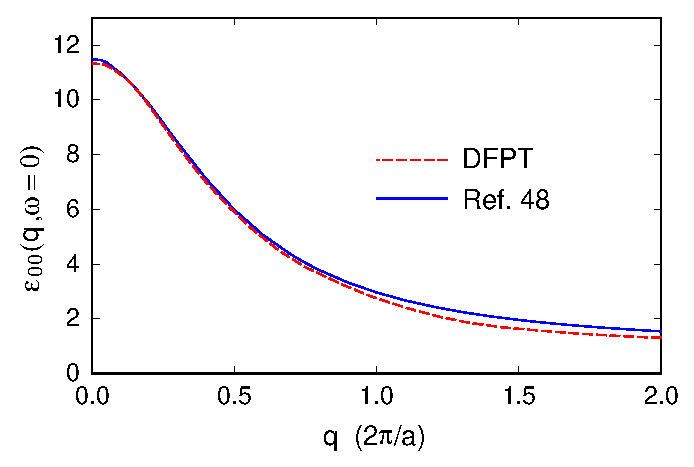
\includegraphics[width=7.5cm]{fig1.eps}
\end    {center}
\caption{\label{fig.pade}
        Comparison of the dielectric function calculated for silicon 
        on the real axis and the analytically continued function starting
        from imaginary frequencies. The three panels correspond to the
        cases illustrated in Fig.\ 3 of Ref.\ \onlinecite{hl86}.
        }
\end    {figure}

\section{Simultaneous calculation of the susceptibility at multiple frequencies}\label{app.multishift}

The linear system given by Eq.\ (\ref{eq.linsys.1}) 
can also be solved efficiently by using a ``multishift'' 
{\tt cBiCG} method.\cite{frommer} 
Multishift methods exploit the knowledge gained during the iterative
solution of the ``seed'' system $Ax=b$ in order to determine the solutions 
of the ``shifted'' system $Ax+\w x=b$, without adding to the the computational 
cost. The logic behind such method is that the seed system and the
shifted system share the same Krilov subspaces $\{b,Ab,A^2b,\cdots\}$,
therefore the residuals of the seed and of the shifted
systems can be taken to be collinear.\cite{frommer}

In practice we can determine the
full frequency-dependent susceptibility 
by performing one single static calculation for each $\q$, $\G$, and $\Gp$.
For the seed system the algorithm is still given by Eqs.\ (\ref{eq.cg1})-(\ref{eq.cg7}).
For the shifted system we replace the calculation of the residuals
$r_{n,\w}$ and of the coefficients $\alpha_{n,\w}$, $\beta_{n,\w}$ by the following relations:
  \begin{equation} \label{eq.shift.1}
  r_{n,\w}  =\frac{r_n}{\pi_{n,\w}};
  \hspace{0.2cm}
  \alpha_{n,\w}  =  \frac{\pi_{n,\w}}{\pi_{n+1,\w}}\alpha_n ;
  \hspace{0.2cm}
  \beta_{n,\w}  =  \Big(\frac{\pi_{n,\w}}{\pi_{n+1,\w}}\Big)^2\beta_n,
  \end{equation}
where the scaling factor $\pi_{n+1,\w}$ is calculated through the recurrence relation
  \begin{equation}\label{eq.shift.2}
  \pi_{n+1,\w} = (1+\w\alpha_n) \pi_{n,\w} + \frac{\alpha_n\beta_{n-1}}{\alpha_{n-1}}(\pi_{n,\w}-\pi_{n-1,\w}).
  \end{equation}
In order to guarantee the collinearity of the residuals, the method
is initialized with $x_0=0$.
The use of Eqs.~(\ref{eq.shift.1}) and (\ref{eq.shift.2}) allows us to
skip the time-consuming operations involving the Hamiltonian in
Eqs.\ (\ref{eq.cg1}) and~(\ref{eq.cg5}).
This method is extremely convienient for determining the frequency-dependent
susceptibility for many frequencies at the cost of one single frequency calculation.
Nevertheless the method presents some practical limitations.

The first major limitation is that the rhs $b$ of the linear system $Ax+\w x=b$
must be the same for all the frequencies considered. In our case
the rhs corresponds to the self-consistent screened perturbation, 
and does depend on the frequency. Therefore if we want to use the
shifted {\tt cBiCG} method we also need to abandon the idea of 
calculating self-consistently the screened Coulomb interaction. 
Instead, we would need to replace this 
by the non-selfconsistent calculation of the susceptibility, followed 
by the explicit inversion of the dielectric matrix for each frequency.
The resulting method constitutes an improved version of the technique
already proposed in Ref.\ \onlinecite{reining}.

The second important limitation is that the shifted {\tt cBiCG} methods
does not allow for the use of effective preconditioners. In fact,
after preconditioning the seed system $M^{-1}Ax=M^{-1}b$ and the shifted
system $M^{-1}Ax+\w M^{-1}x=M^{-1}b$ no longer share the same Krilov subspaces, 
hence the residuals are no longer collinear.\cite{simoncini} 
The practical consequence is that for systems with
large basis set energy cutoffs and small band gaps, the number of iterations
required to achieve convergence can be extremely large.
In addition, the convergence rate of the shifted method is dictated
by the worst-conditioned system, therefore also in this case
we need to perform calculations along the imaginary axis and then anaytically
continue the function to real frequencies.

If we consider that we need approximately 10 frequency points for the
Pad\'e approximants, and each preconditioned calculation requires
in average approximately 10 iterations and 5 self-consistency cycles, 
we conclude that the direct calculation of the screened Coulomb interaction
will be convenient as long as the (non-preconditioned)
shifted {\tt cBiCG} method requires more than $10\times10\times5=500$ 
iterations (assuming that the cost of matrix inversion is negligible).
On the other hand, if we need an ultra-fine sampling of the frequency
dependence, then the shifted method would prove advantageous.

\section{Calculation of the Green's function using Haydock's recursion method}\label{app.haydock}

\begin{thebibliography}{99}

\bibitem{hl}
L. Hedin and S. Lundqvist,
Effects of the electron-electron and the electron-phonon interaction in
the one-electron states of solids,
in {\it Solid State Physics}, ed. by F. Seitz, D. Turnbull, and
H. Ehrenreich, (Academic, New York, 1969), vol.\ 23, pag. 1.

\bibitem{hl86}
M. Hybertsen and S. G. Louie, 
Phys.\ Rev.\ B {\bf 34}, 5390 (1986).

\bibitem{painless.cg}
G.\ H.\ Golub and C.\ F.\ Van Loan, {\it Matrix Computations} (John Hopkins University Press, Baltimore, 1983).

\bibitem{jacobs}
D.\ A.\ H.\ Jacobs,
IMA J.\ Numer.\ Anal.\ {\bf 6}, 446 (1986).

\bibitem{baroni.rmp}
S. Baroni, S. de Gironcoli, A. Dal Corso, and P. Giannozi, 
Rev.\ Mod.\ Phys.\ {\bf 73}, 515 (2001).

\bibitem{tpa}
M. P. Teter, M. C. Payne, and D. C. Allan,
Phys.\ Rev.\ B {\bf 40}, 12255 (1989).

\bibitem{pade1}
K.-H. Lee and K. J. Chang,
Phys.\ Rev.\ B {\bf 54}, R8285 (1996).

\bibitem{pade2}
H. J. Vidberg and J. W. Serene,
J.\ Low.\ Temp.\ Phys.\ {\bf 29}, 179 (1977).

\bibitem{pade3}
S. Leb\`egue, B. Arnaud, M. Alouani, and P. E. Bloechl,
Phys.\ Rev.\ B {\bf 67}, 155208 (2003).

\bibitem{godby1}
H. N. Rojas, R. W. Godby, and R. J. Needs,
Phys.\ Rev.\ Lett.\ {\bf 10}, 1827 (1995).

\bibitem{nelder-mead}
J. A. Nelder and R. Mead, 
Comput. J. {\bf 7}, 308 (1965).
We used the implementation available from the
{\tt E04CCF} routine of the {\tt NAG} library
({\tt www.nag.co.uk}).

\bibitem{frommer}
A. Frommer,
Computing {\bf 70}, 87 (2003).

\bibitem{reining}
L. Reining, G. Onida, and R. W. Godby, 
Phys.\ Rev.\ B {\bf 56} R4301 (1997).

\bibitem{simoncini}
V. Simoncini and D. B. Szyld,
Numer.\ Linear Algebr.\ {\bf 14}, 1 (2006).

\bibitem{balde_tosa}
A. Baldereschi and E. Tosatti,
Phys.\ Rev.\ B {\bf 17}, 4710 (1978).

\bibitem{cohen_berg}
M. L. Cohen and T. K. Bergstresser,
Phys.\ Rev.\ {\bf 141}, 789 (1966).

\bibitem{baroni-resta}
S. Baroni and R. Resta,
Phys.\ Rev.\ B {\bf 33}, 7017 (1986).

\bibitem{degironcoli}
S. de Gironcoli,
Phys.\ Rev.\ B {\bf 51}, 6773 (1995).

\bibitem{hl86-prb}
M. S. Hybertsen and S. G. Louie,
Phys.\ Rev.\ B {\bf 35}, 5585 (1976).

\bibitem{cpm}
R. M. Pick, M. H. Cohen, and R. M. Martin,
Phys.\ Rev.\ B {\bf 1}, 910 (1970). 

\bibitem{kunc}
K. Kunc and E. Tosatti,
Phys.\ Rev.\ B {\bf 29}, 7045 (1984).

\bibitem{oxfordgw}
Borrowing some subs from espresso - developed by FG - will become
GNU - need to be ported to main packages.

\bibitem{alavi}
J. Spencer and A. Alavi.
Phys.\ Rev.\ B {\bf 77} 193110 (2008).

\bibitem{marzari}

\bibitem{haydock1}

\end{thebibliography}

\end{document}
